We collected nouns taking sentential complements from the Penn Treebank (English) and the Universal Dependencies treebanks (German and Spanish).



\begin{figure}
    \centering
    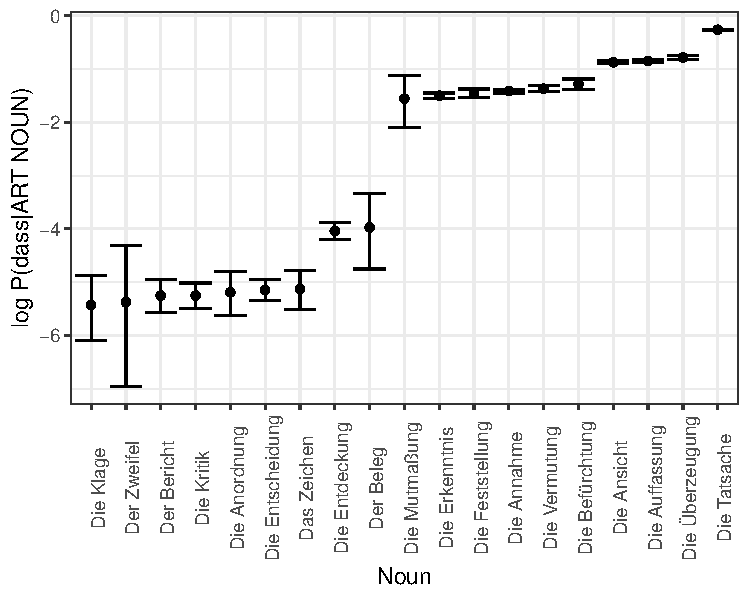
\includegraphics[width=0.4\textwidth]{../resource-rational-surprisal/materials/nouns/figures/nouns_german.pdf}
    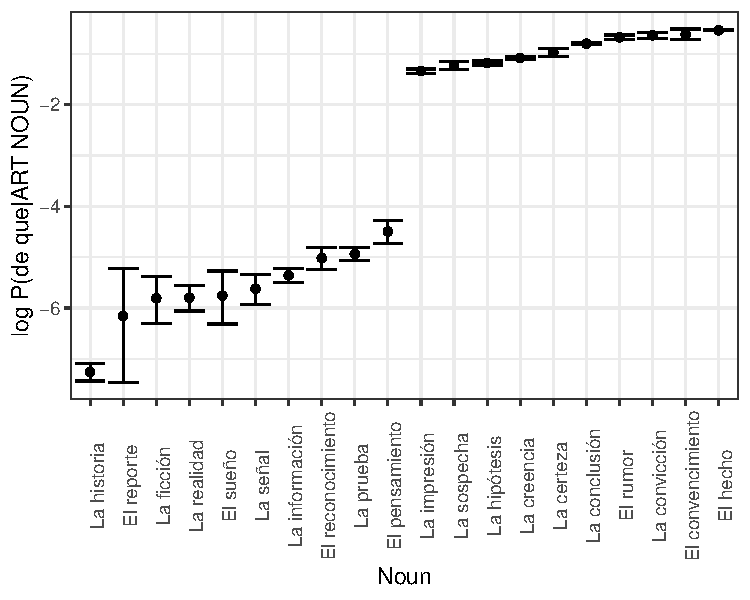
\includegraphics[width=0.4\textwidth]{../resource-rational-surprisal/materials/nouns/figures/nouns_spanish.pdf}

	\caption{Nouns in German and Spanish selected for Experiment 3, with Embedding Bias and a 95\% binomial confidence interval.}
    \label{fig:german-spanish-nouns}
\end{figure}



\begin{figure}
	\centering
	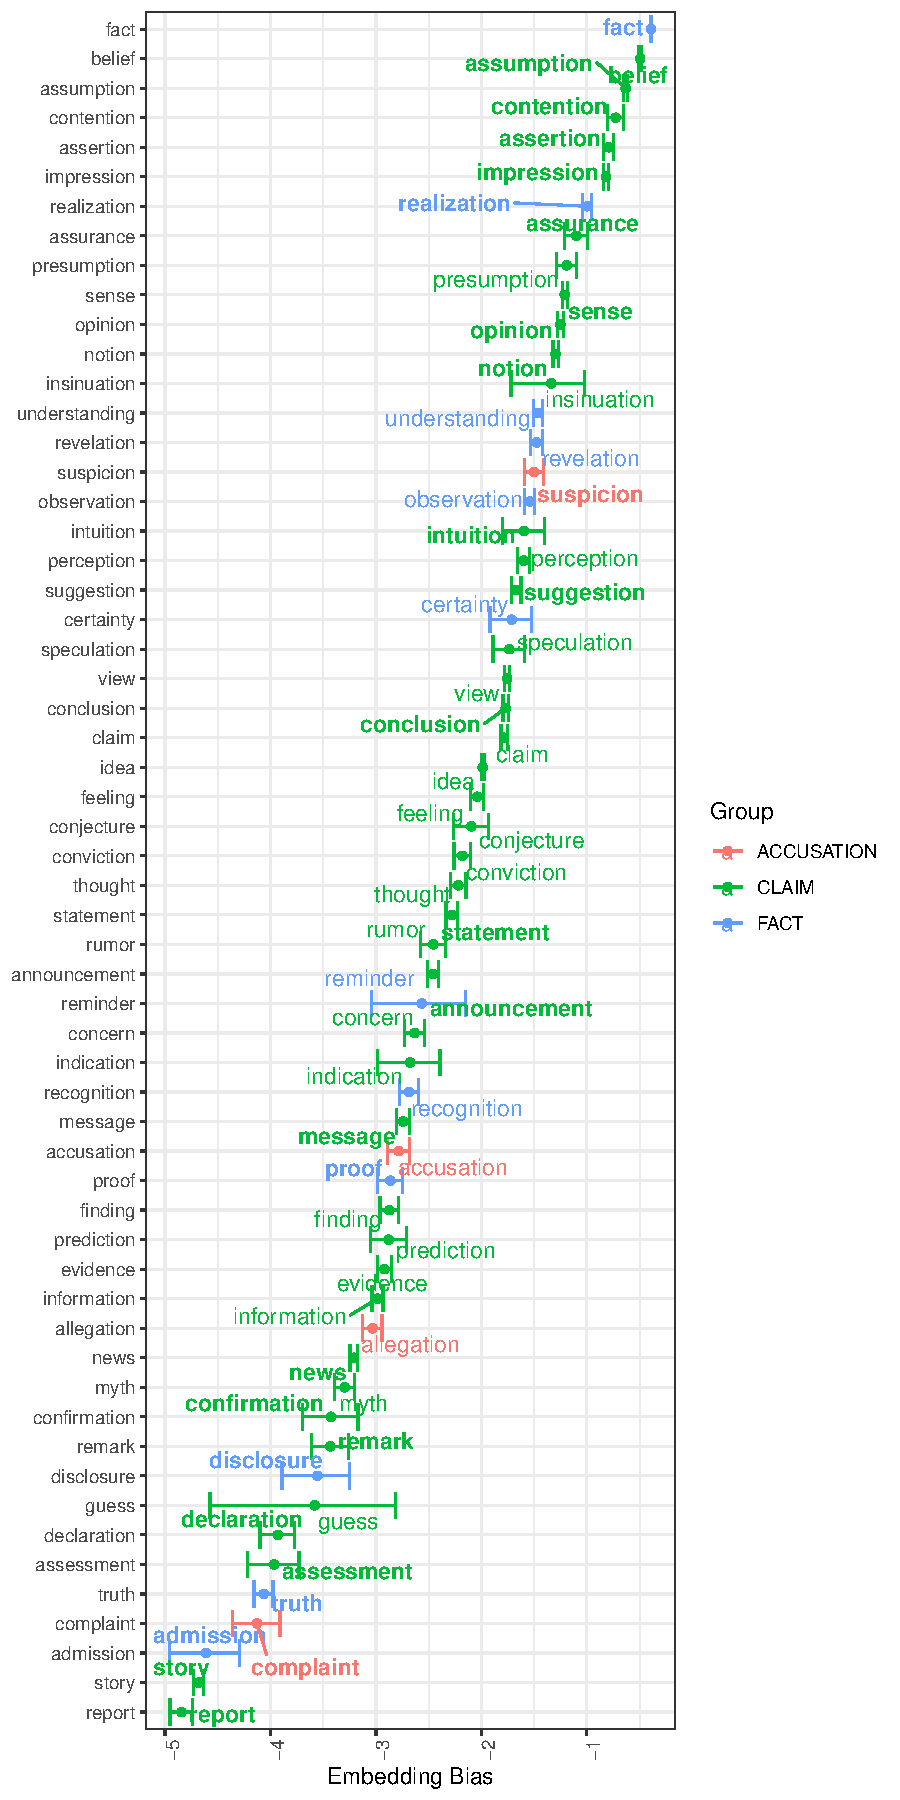
\includegraphics[width=0.6\textwidth]{../resource-rational-surprisal/materials/nouns/English/figures/All_nouns_byType.pdf}

	\caption{English nouns by Embedding Bias as estimated on Wikipedia, annotated for the three semantic classes. This plot contains all 58 nouns considered in model simulations. Nouns used in Experiments 1--2 are marked in bold. We show 95\% binomial confidence intervals for embedding bias.}\label{fig:english-nouns}
\end{figure}



\begin{figure}
	\centering
	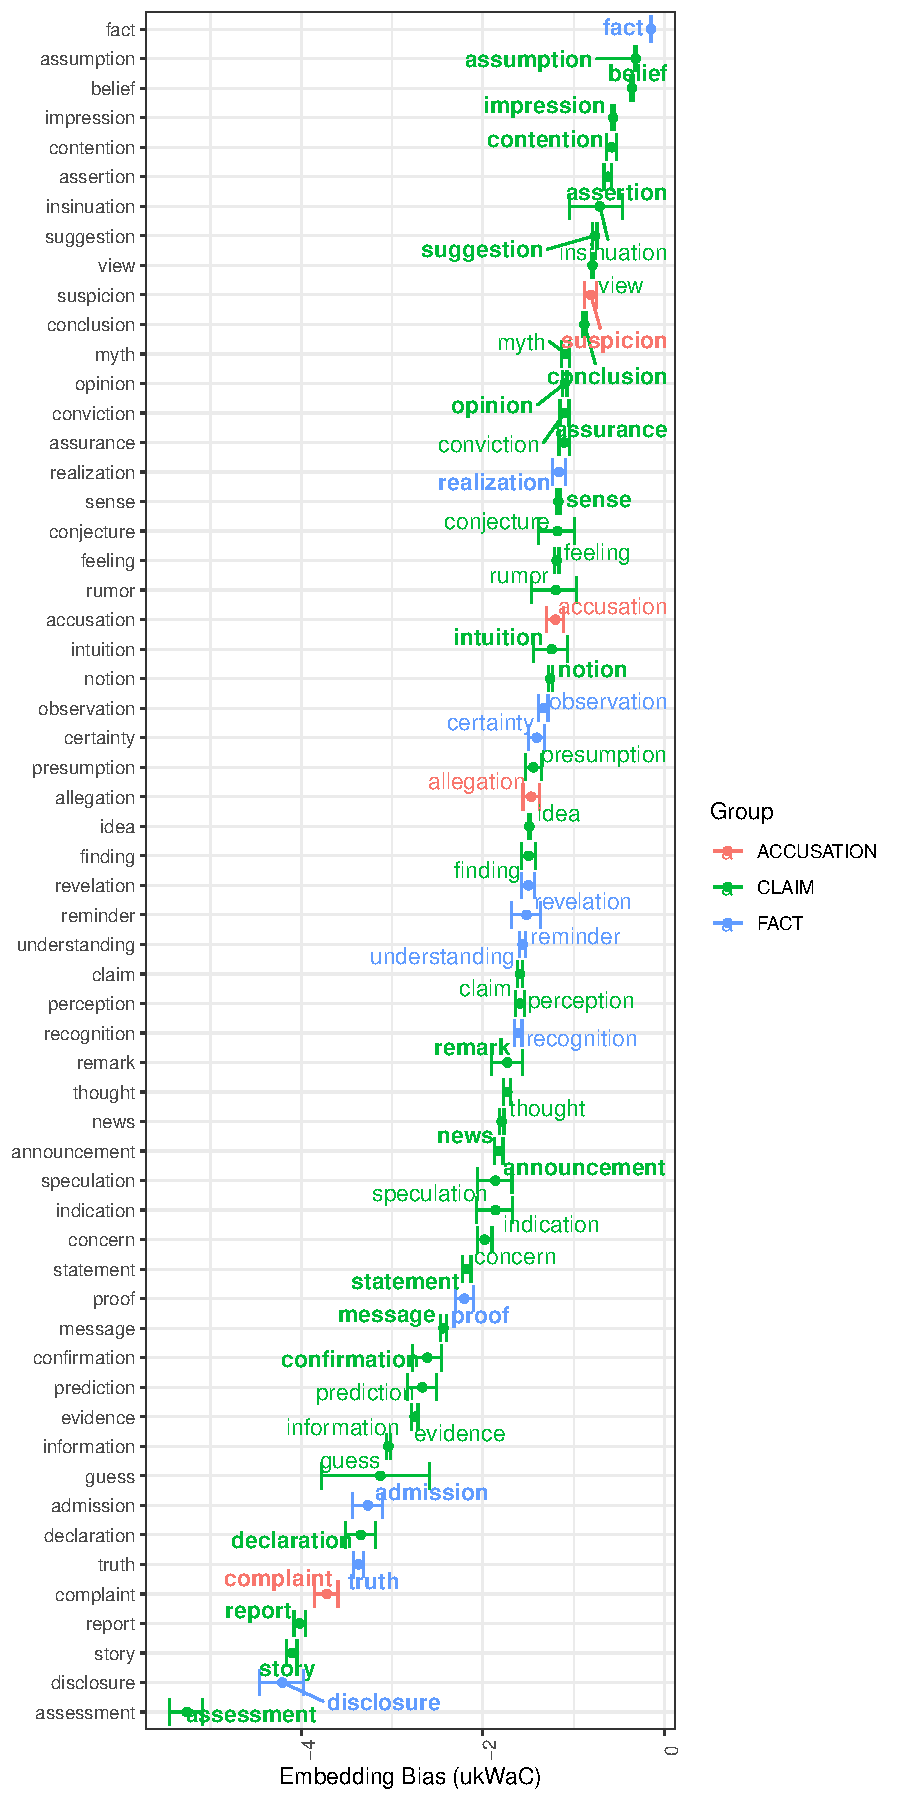
\includegraphics[width=0.45\textwidth]{../resource-rational-surprisal/materials/nouns/English/figures/All_nouns_byType_ukWaC.pdf}
	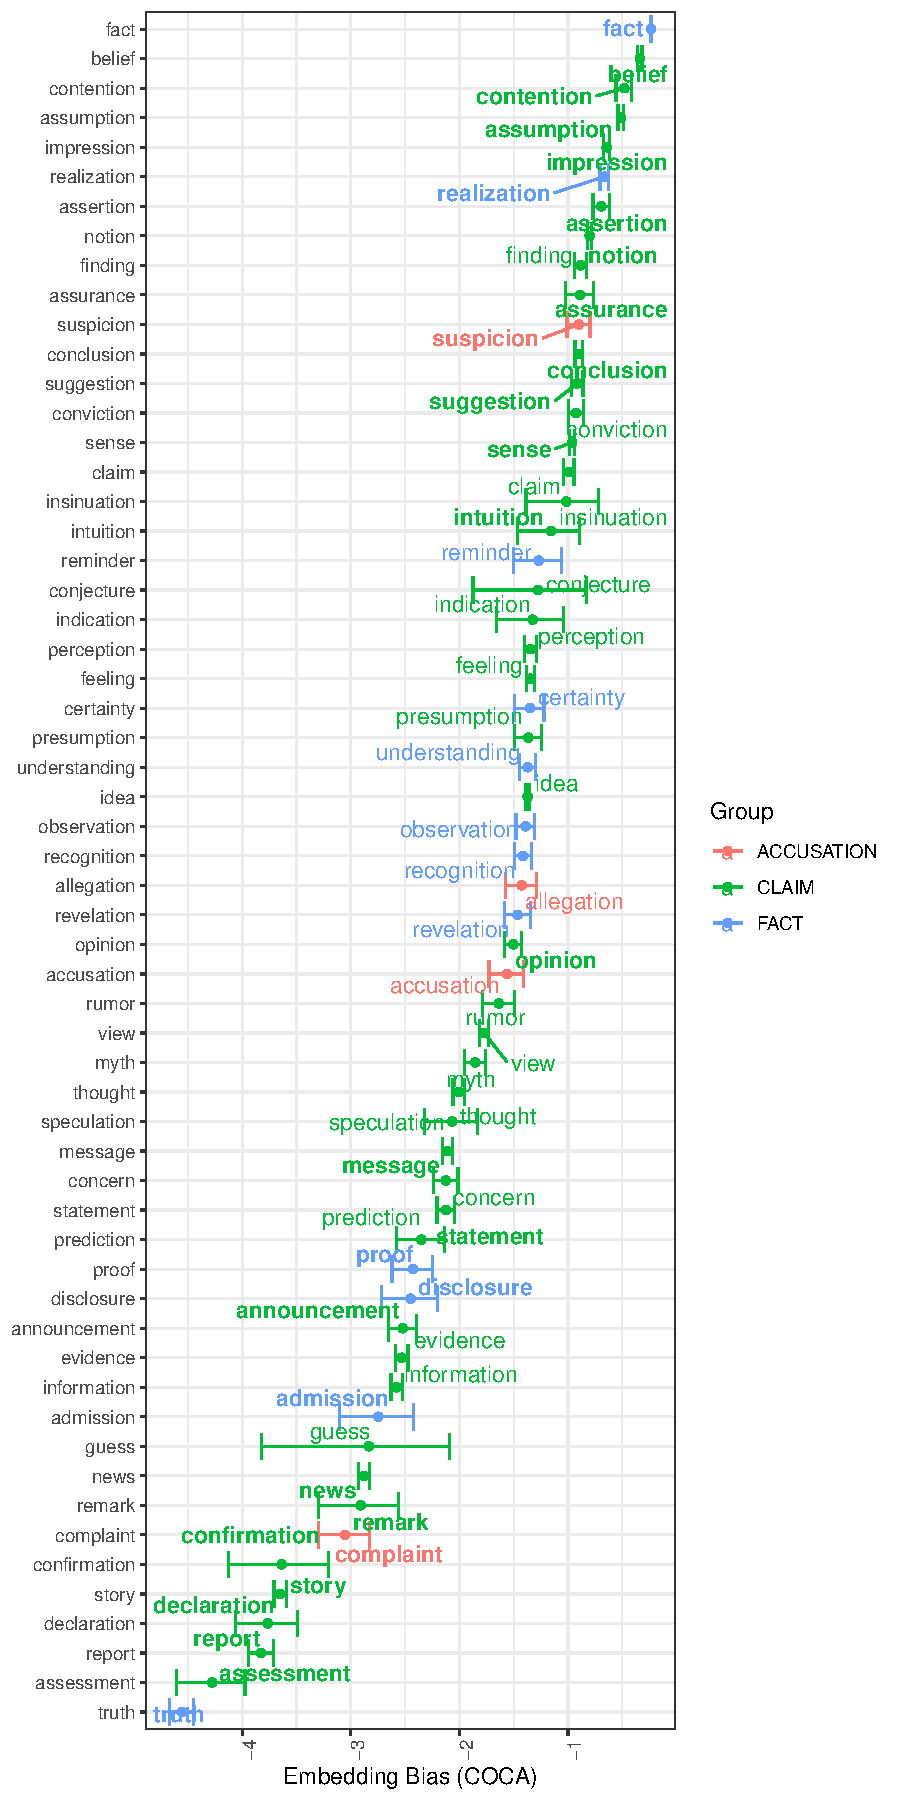
\includegraphics[width=0.45\textwidth]{../resource-rational-surprisal/materials/nouns/English/figures/All_nouns_byType_COCA.pdf}

	\caption{English nouns by Embedding Bias as estimated on ukWaC and COCA (see Section~\ref{sec:embedding-rate-other-corpora}). Compare Figure~\ref{fig:english-nouns}.}\label{fig:english-nouns-ukwac-coca}
\end{figure}



\paragraph{English}
From an initial set of 161 English nouns labeled as embedding a complement clause in the Penn Treebank, we selected 58 nouns based on overall semantic fit with the items.
While we used all 58 nouns in model simulations, the behavioral experiments focused on nouns with very low and very high embedding bias to maximize statistical precision.

We estimated embedding bias using Wikipedia; see Section~\ref{sec:embedding-rate-other-corpora} for results using two other large corpora for estimating Embedding Bias.
Note that, in English, \emph{that} can embed both complement clauses and relative clauses; Embedding Bias does not distinguish between those different types of embedded clauses.
We also evaluated nouns' biases specifically towards complement clauses in Section~\ref{sec:other-possible-predictors}, finding that the nouns under consideration tend to be strongly biased towards complement clause embedding as opposed to relative clause embedding.
In that section, we also investigated whether separately considering a noun's bias to embed complement or relative clauses predicts human reading times beyond Embedding Bias, finding little, if any, evidence for such effects.

\paragraph{Semantic Grouping}
In order to eliminate any item-specific confounds, we cross nouns with items across subjects in the reading time studies.
This raises the question of how to deal with combinations that are semantically infelicitous, which primarily happens with nouns that presuppose truth of the embedded proposition -- e.g., the combination ``fact'' + ``was false'' tends to be semantically infelicitous\footnote{We note that such combinations typically still are felicitous in certain contexts, e.g. \textit{Everyone else tries to guess whether they think the \textbf{fact was false}.} \url{https://medium.com/future-of-design-in-higher-education/zoom-friendly-warmups-and-icebreakers-3400c8b7263}; \textit{If they only discovered that the \textbf{fact was a lie} after the wedding} \url{https://www.catebrough.com/can-i-have-my-south-carolina-marriage-annulled/}.}

We therefore grouped nouns into three classes and annotated the items for compatibility with those, matching only compatible pairs.
We distinguished entailing and non-entailing nouns, as defined by \cite{huddleston2002the}. We further distinguished \textit{claim}-like and \textit{accusation}-like nouns to account for a group of items that presuppose positive valence (e.g., ``the NOUN that the paramedic saved the children...''), making them less compatible with \textit{accusation}-like nouns.
This leads to the following three classes.
\begin{enumerate}
	\item Entailing nouns  (e.g., fact).
    \item Claim-like non-entailing nouns (e.g., claim, report).
    \item Accusation-like non-entailing nouns (e.g., accusation, allegation).
\end{enumerate}

See Figure~\ref{fig:english-nouns} for the full list of nouns used in simulations and studies with this annotation.


Note that we on purpose did not aim to only include high-plausibility combinations.
Rather, our goal was to eliminate semantic anomalies where an entailment presupposition is violated. 
While it would be possible to consider the \emph{plausibility} or \emph{frequency} of a noun-verb match, this would introduce additional probabilistic biases into the noisy-channel reasoning that could confound the effect of theoretical interest, i.e., the Embedding Bias effect.


\paragraph{German and Spanish}
In German and Spanish, we selected 20 nouns based both on semantic fit with the nouns used in the English experiments, and focused on extreme values of complement clause bias to maximize power in the production studies.
Resulting nouns are shown in Figure~\ref{fig:german-spanish-nouns}.

We note that, in the Spanish study, due to a scripting error not discovered before data analysis, the noun \textit{pensamiento} was not included in the experiment, resulting in only 19 nouns.


Whereas ``the NOUN that'' allows both sentential complement and relative clause continuations in English, German and Spanish use complementizers (\textit{dass} and \textit{de que}) that are used only for complement clauses, not used for relative clauses.

